\documentclass{article}

\usepackage{amsmath, amssymb}
\usepackage{geometry}[margin=1in]
\usepackage{enumitem}
\usepackage{pdfpages}

\author{Isaac Boaz}
\title{CSCI 447 Homework 4}

\begin{document}
\maketitle

\section*{Question 1}
For an average page fault service of 5 milliseconds, and a memory access time of
300 nanoseconds, what is the maximum access(es) out of 2,000 attempts that can
cause a page fault so that the effective access time is \emph{at most} 6.6 microseconds?

\begin{align*}
    \frac{5,000,000 \cdot n + 300 \cdot (2,000 - n)}{2,000} & \leq 6,600                          \\
    5,000,000n + 600,000 - 300n                             & \leq 13,200,000                     \\
    4,999,700n                                              & \leq 12,600,000                     \\
    n                                                       & \leq \frac{12,600,000}{4,999,700}   \\
    n \leq 2                                                & \text{ acceses causing page faults}
\end{align*}

\section*{Question 2}
Given the following page requests:
\texttt{1, 2, 3, 4, 2, 1, 5, 6, 2, 1, 2, 3, 7, 6, 3, 2, 1, 2, 3, 6}

Regardless of the eviction algorithm used, if we are only given 1 frame of memory,
since there are no duplicate page requests (e.g. 1, 1), the number of page faults
is equal to the number of page requests (i.e. \textbf{20}).

Similarly, since there are only 7 unique pages being requested, with 7 frames of
memory we will always have a page fault on the first unique 7 pages, and no page
faults on the remaining requests. Thus, the number of page faults is \textbf{7}.

Sadly we need to do more work for the 3 and 5 frame cases.

\begin{tabular}{c|cc}
    Strategy & 3 Frames & 5 Frames \\
    \hline
    LRU      & 15       & 8        \\
    FIFO     & 16       & 10       \\
    Optimal  & 11       & 7
\end{tabular}

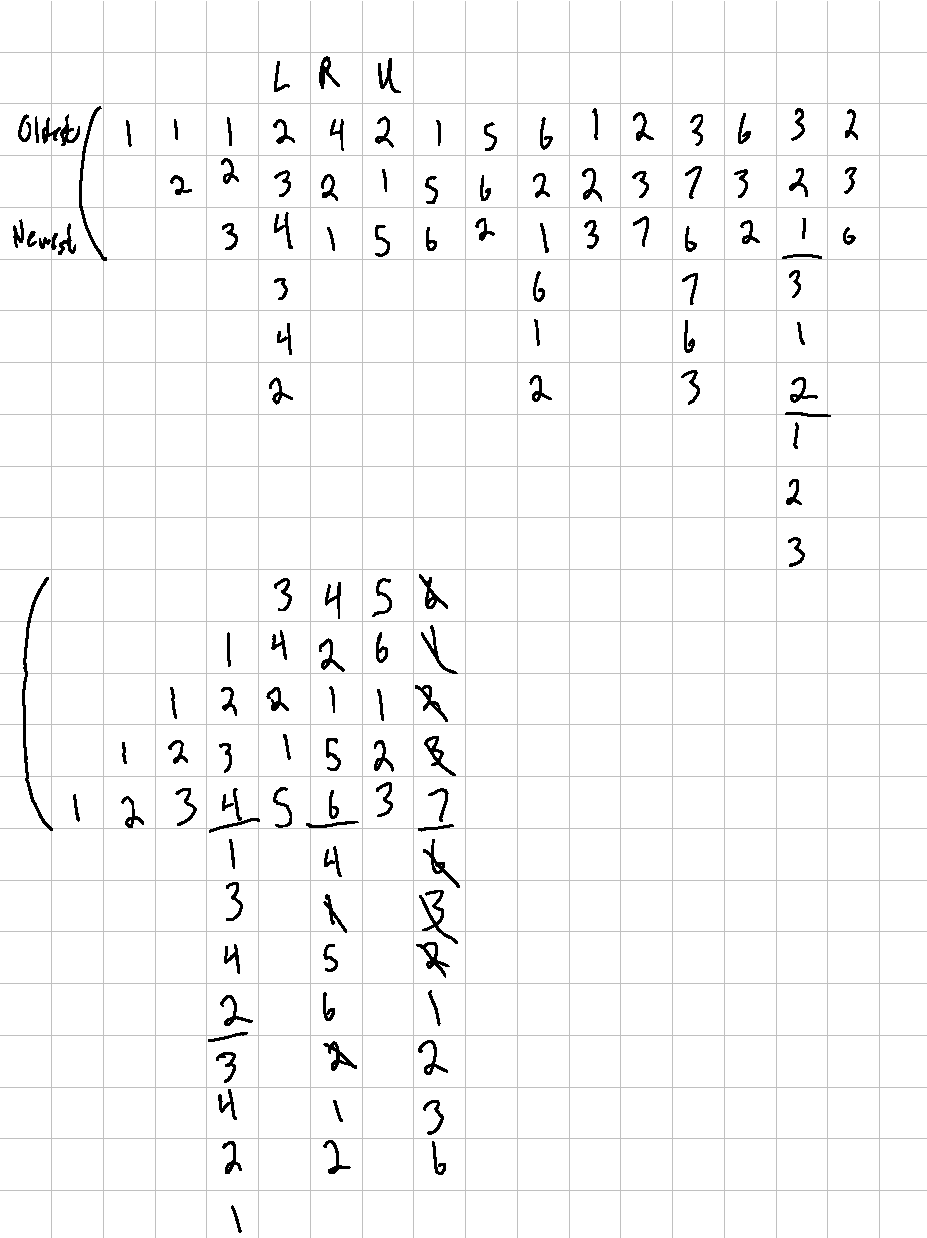
\includegraphics[scale=0.5,page=1]{Q2.pdf}
\includegraphics[scale=0.5,page=2]{Q2.pdf}
\includegraphics[scale=0.5,page=3]{Q2.pdf}

\section*{Question 3}
\begin{itemize}
    \item Faster CPU: Most likely not, as the CPU utilization is already low, and it appears the bottleneck is the paging disk.
    \item Install a bigger paging disk: This would likely help, as it would
          increase the number of pages that can be stored in memory, reducing the
          number of page faults.
    \item Increase the degree of multiprogramming: This could help, as it would
          allow the CPU to switch to another process while waiting for either the I/O
          or the paging disk.
    \item Decrease the degree of multiprogramming: This could help in a rare
          case if switching between processes is causing a significant amount of
          overhead (either due to limited memory or many page faults).
    \item Install more main memory: This would likely help, as it would reduce the
          number of page faults.
    \item Install a faster hard disk or multiple controllers with multiple hard disks: This would likely help, as it would reduce the time spent waiting for the paging disk.
    \item Increase the page size: This could help, since the I/O device is only at 5\% utilization, it is likely that the bottleneck is the paging disk.
\end{itemize}
\end{document}